\documentclass{article}
\usepackage{amsmath}
\usepackage{amsthm}
\usepackage{amssymb}
\usepackage{commath}
\newtheorem{theorem}{Theorem}
\usepackage{hyperref}
\usepackage{graphicx}
\DeclareMathOperator{\ex}{ex}
\begin{document}
This compiles results from:
\begin{itemize}
\item Conforti et al.'s survey on extended formulations: \url{http://personal.lse.ac.uk/Zambelli/papers/surveyextended\%20formulations-Feb2010.pdf}
\item Caen on sum of squares of degrees of a graph: \url{http://www.sciencedirect.com/science/article/pii/S0012365X97002136}
\end{itemize}

Let $G=(V,E)$ plane.

\begin{theorem}
	A 1-factor is exactly a $V$-join of size $\abs{V}/2$.
\end{theorem}
\begin{theorem}
Let $T\subseteq V$ with $\abs{T}$ even. The symmetric difference of two $T$-joins is an $\varnothing$-join.
\end{theorem}
\begin{theorem}
Fix two $T$-joins $A\neq B$. There exists an $\varnothing$-join $C$ such that $A = B\bigtriangleup C$.
\end{theorem}
\begin{proof}
Namely, $A\bigtriangleup B$.
\end{proof}

\begin{theorem}
Fix a $V$-join (1-factor) $A$. The $V$-join polytope (for any $G$ not necessarily planar) is

$$P^{\text{$V$-join}}(G) = \cbr{y\in \mathbf{R}^E: \text{there exists $x\in P^{\text{$\varnothing$-join}}(G)$, $y_e = x_e$ for all $e\not\in A$ and $y_e=1-x_e$ for all $e\in A$}}$$
\end{theorem}

\begin{theorem}
The $\varnothing$-join polytope (for any $G$ not necessarily planar) is

$$P^{\text{$\varnothing$-join}}(G) = \cbr{x\in\mathbf{R}^E: \begin{array}{ll}
x(F)-x(\delta(S)-F) \leq \abs{F}-1 & S\subsetneqq V, \text{$S$ a minimal cut}, F\subseteq \delta(S), \abs{F}\text{ odd} \\
0\leq x\leq 1 &
\end{array}}$$
\end{theorem}

\begin{theorem}
A 2-factor is a $\varnothing$-join with every vertex having degree 2.
\end{theorem}

\begin{theorem}
Let $G$ be planar and $G^*$ a planar dual. $S\subseteq E$ is a $\varnothing$-join (equivalently, an Eulerian spanning subgraph; a disjoint union of cycles; a member of the cycle space $\mathcal{C}(G)$) if and only if $S^*$ is a cut of $G^*$. Additionally,
$S$ is a simple cycle if and only if $S^*$ is an (inclusion-) minimal cut.
\end{theorem}

\begin{theorem}
Let $G$ be a graph not necessarily planar.
Let $P^{cut}(G)$ denote the convex hull of cuts of $G$. Then $P^{cut}(G)$ is a subset of:

$$ R(G) = \cbr{x\in \mathbf{R}^E: \begin{array}{ll}
x(F)-x(C-F)\leq \abs{F}-1 & C\in \mathcal{C}(G), F\subseteq C, \abs{F}\text{ odd} \\
0\leq x\leq 1
\end{array}}$$

\end{theorem}

\begin{theorem}
For planar graphs (and some others), $P^{cut}(G) = R(G)$.
\end{theorem}

\begin{theorem}
Let $G=(V,E)$ planar.
For $x\in \cbr{0,1}^E$, let $x^*\in\cbr{0,1}^{E^*}$ be the characteristic
vector of the dual edges. Then
$$P^{\text{$\varnothing$-join}}(G) = \cbr{x\in\mathbf{R}^E: x^*\in P^{cut}(G^*)} = \cbr{x\in\mathbf{R}^E: x^*\in R(G^*)}$$
\end{theorem}

\begin{proof}
If $x^* \in P^{cut}(G^*)$, then $x^*(F)-x^*(C-F)\leq \abs{F}-1$ for every $C\in \mathcal{C}(G^*)$ and odd size $F\subseteq C$. In particular this holds for every circuit $C\subseteq E^*$. By circuit-minimal cut duality, the corresponding inequality holds for the minimal cut $C^*\subseteq E$ in the primal graph.
\end{proof}


\begin{theorem}
Let $G=(V,E)$ be planar. Let $H=(V, E')$ with $E\subseteq E'$. Then $R(G)$ is the projection of $R(H)$ onto $\mathbf{R}^E$.
\end{theorem}

\begin{theorem}
Let $C$ be a cycle with a chord. Then the cut inequality for $C$ is implied by the inequalities for the cycles on either side of the chord. 
\end{theorem}

\begin{theorem}
Let $H$ be a complete triangulation (i.e. every facial cycle is a triangle) of $G$. Then  $R(H)$ is a compact formulation for $R(G)$.
\end{theorem}
\begin{proof}
Triangles are the only cycles without chords. So
the only cut inequalities needed are the ones for triangles. 
There are only $O(V)$ triangles in a planar triangulated graph since the number of faces is $O(V)$. 
\end{proof}


\begin{theorem}
Fix a $V$-join $A$.
Let $E^\Delta\supseteq E^*$ so that $(V^*, E^\Delta)$ is triangulated.
The following (with the projection map onto $y$) is a compact formulation for $P^{\text{V-join}}(G)$

$$\cbr{(y,x,z)\in\mathbf{R}^E\times\mathbf{R}^E\times\mathbf{R}^{E^\Delta-E}:
\begin{array}{lr}
y_e = x_e & e\not\in A \\
y_e = 1-x_e & e\in A \\
	(x,z)(F) - (x,z)(C-F) \leq \abs{F}-1 & \text{triangle $C \subseteq E^\Delta$ in $(V,E^\Delta)$} \\
0 \leq y,x,z \leq 1
\end{array}
}$$
\end{theorem}

\begin{theorem}
A compact formulation for the 1-factor polytope of $G$ is:
	$$\cbr{(y,x,z) \in P^{\text{$V$-join}}(G): \mathbf{1}^Ty = \abs{V}/2}$$
\end{theorem}
\begin{proof}
	Every $V$-join has size at least $\abs{V}/2$. Hence,
	the above polyhedron is integer since it is a face of $P^{\text{$V$-join}}(G)$.
\end{proof}

	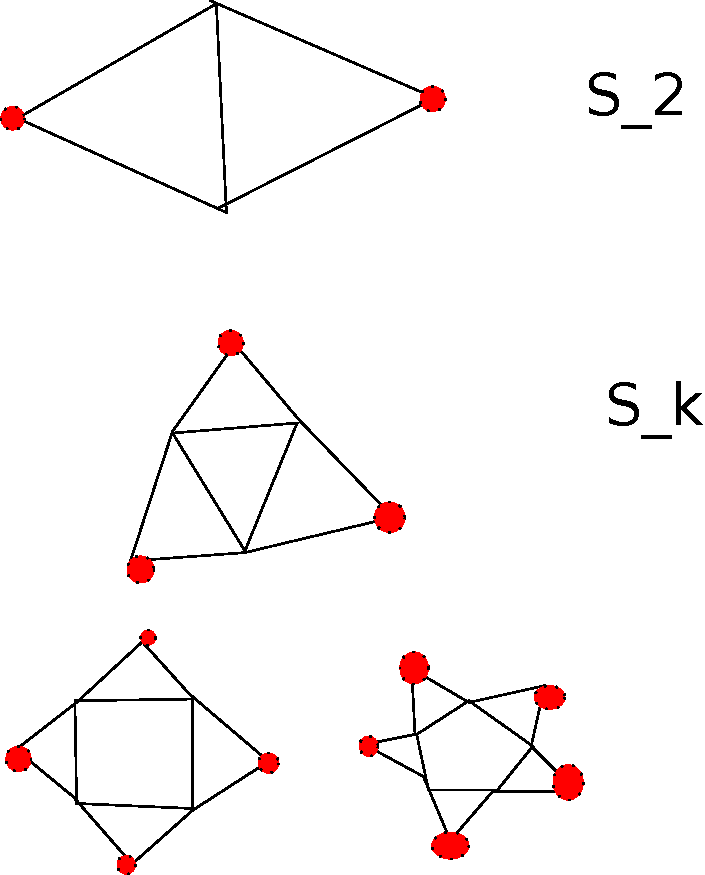
\includegraphics[width=0.5\textwidth]{gadgets}

	\begin{theorem}
		Let $k\geq 2$ integer. Let $0\leq \ell \leq k$ integer.
		Let $T$ be a set of red vertices of $S_k$ with $\abs{T} =\ell$.
		Then $S_k - T$ has 1-factor if and only if $\ell$ is even.
	\end{theorem}

	\begin{proof}
		First, assume $k=2$. By inspection, $S_2$ has a 1-factor. If 
		$\ell=1$, then $S_2 - T$ is a triangle, which has no 1-factor.
		If $\ell=2$, then $S_2 - T$ is a single edge, which has a 1-factor.
		This completes the proof for $k=2$.

		Now, assume $k>2$. Let $C$ be the unique induced cycle of $S_k$
		with no red vertices. Call an induced triangle a \emph{red triangle}
		if it contains a red vertex. $S_k - T$ has $k-\ell$ red triangles.
		
		Let $\ex(G)$ be the minimum number of vertices not saturated
		by a matching of $G$.
		For an odd cycle $C$ in $G$, let $G/C$ denote the contraction of $C$
		to a point.  
		Recall that for any odd cycle $C$, $\ex(G) \leq \ex(G/C)$.

		Let $H$ be $S_k - T$ with all red triangles contracted.
		Then $H$ is a cycle of length $k - (k-\ell) = \ell$.

		If $\ell$ is even, then the cycle $C_\ell$ has a 1-factor.
		Hence, $S_k - T$ has a 1-factor. 

		If $\ell$ is odd, then since $S_k - T$ has $2k - \ell$ vertices
		and $2k-\ell$ is odd, $S_k - T$ has no 1-factor.
	\end{proof}


	Assume every vertex of $G$ has degree at least two.
	Let $G' = (V\sqcup V^\dagger, E\sqcup E^\dagger)$ be $G=(V,E)$
	with each vertex $v$ of degree $k$ replaced with the gadget $S_k$,
	with the edges in $\delta(v)$ connected to $v$'s gadget at the red vertices.


	Then $G$ has an $\varnothing$-join if and only if $G'$ has a 1-factor.
	
	So, $G$ has a 2-factor if and only if $G'$ has a 1-factor that,
	for each vertex $v\in V$,
	uses two original edges from $\delta_G(v)$.

	
	Hence, given a triangulation $E^\Delta\supseteq E(G')$ of $G'$,
	the following polyhedron (with the projection map
	on $y$) contains the 2-factor polytope  of $G$:

	$$\cbr{(y,a,x,z)\in \mathbf{R}^{E}\times\mathbf{R}^{E^\dagger} \times \mathbf{R}^{E \sqcup E^\dagger} \times \mathbf{R}^{E^\Delta - (E\sqcup E^\dagger)} : \begin{array}{ll}
		((y,a),x,z) \in P^{\text{$V$-join}}(G') \\
		\mathbf{1}^T(y,a) = \abs{V\sqcup V^\dagger} / 2 \\
		y(\delta_G(v)) = 2& v\in V \\
		0\leq y,a,x,z \leq 1
	\end{array}} $$

	It may not be integral unless $y(\delta_G(v)=2)$ only
	intersects $P^{\text{1-factor}}(G')$ at its vertices.

	...Then I might as well say that the 2-factor polytope is contained
	in the following polyhedron:

	$$\cbr{x\in P^{\text{$\varnothing$-join}}(G) : \begin{array}{ll}
		x(\delta(v)) = 2 & v\in V
	\end{array}} = \cbr{x \in \mathbf{R}^E: \begin{array}{ll}
		x^* \in R((V^*, E^\Delta)) \\
		x(\delta(v)) = 2
	\end{array}}$$

\end{document}
